\section{How well it does}\label{sec:results}

This section compares DFG with the networks and every other reference: on the held-out suite, on all 11 toy suites, against v3 and the low-degree algorithm, in the input dimension, on tabular data and in compute. Numbers come from \repo{study/part11/RESULTS.json}, which \repo{study/part11/compare_dfg.py} computes from the result files, unless another file is named; the tables and figures are generated from it by \repo{paper_dfg/make_tables.py} and \repo{paper_dfg/make_figures.py}, and derived numbers that no table shows are in \repo{paper_dfg/tables/numbers.json} and the figures' \texttt{.json} files. The rules are those of \cref{sec:metrics}; \cref{app:further} gives every target and the further comparisons.

% ------------------------------------------------------------------------------------------------------------------
\subsection{The held-out suite \code{dlheld7}}\label{sec:res-dlheld7}

\code{dlheld7} is the only toy suite held out for DFG v1.3 (\cref{sec:part11}). \Cref{tab:dlheld7} gives every target's definition and $\nstar$, and \cref{tab:dlheld7-summ} (\cref{app:further-targets}) the summaries against each reference.

\begin{table}[t]
\centering{\footnotesize\setlength{\tabcolsep}{3pt}\renewcommand{\arraystretch}{1.1}
\begin{tabularx}{\linewidth}{@{}l>{\raggedright\arraybackslash}Xrrrrrrrrrrr@{}}
\toprule
 & & \multicolumn{3}{c}{discrete, inputs permuted} & \multicolumn{2}{c}{calibration} & \multicolumn{4}{c}{networks} & \multicolumn{2}{c}{\hd{$\log_2$ ratio, DFG\\alone to}}\\
\cmidrule(lr){3-5}\cmidrule(lr){6-7}\cmidrule(lr){8-11}\cmidrule(l){12-13}
target & definition & \hd{DFG\\alone} & v3 & \code{lowdeg} & \code{lin} & \code{hgb} & \hd{\code{nets_}\\\code{wd}} & \hd{\code{nets_}\\\code{cewd0.3}} & \hd{\code{nets_}\\\code{cewd1.0}} & \hd{\code{nets_}\\\code{best}} & \hd{\code{nets_}\\\code{best}} & v3\\
\midrule
f7\_00 & {\scriptsize OR([$|$s1$|$ $\le$ 0],\allowbreak{} [s2 == $-$1]),\allowbreak{} s1 = x1+\allowbreak{}x2\allowbreak{}$-$x3\allowbreak{}$-$x4,\allowbreak{} s2 = $-$x5\allowbreak{}$-$x6\allowbreak{}$-$x7+\allowbreak{}x8+\allowbreak{}x9+\allowbreak{}x10+\allowbreak{}x11} & 211 & \textbf{203} & 7061 & never & 6208 & 2418 & 1545 & 1565 & 1545 & $-2.87$ & $+0.06$\\
f7\_01 & {\scriptsize [s $\le$ 1],\allowbreak{} s = x1+...+\allowbreak{}x13} & 119 & \textbf{106} & 595 & 111 & 684 & 205 & 121 & 119 & 119 & $-0.00$ & $+0.17$\\
f7\_02 & {\scriptsize OR(AND(x2,\allowbreak{}$-$x6,\allowbreak{}$-$x8),\allowbreak{} AND(x1,\allowbreak{}$-$x2,\allowbreak{}$-$x4,\allowbreak{}$-$x5),\allowbreak{} AND(x3,\allowbreak{}$-$x5,\allowbreak{}$-$x7))} & 190 & \textbf{106} & 435 & never & 120 & 337 & 341 & 348 & 337 & $-0.83$ & $+0.85$\\
f7\_03 & {\scriptsize $-$x11 ? [((s1+6)/2) mod 4 != 2] : [$|$s2$|$ > 2],\allowbreak{} s1 = x1+...+\allowbreak{}x6,\allowbreak{} s2 = x7+...+\allowbreak{}x10} & \textbf{352} & 352 & 4205 & never & 2199 & 1710 & 1665 & 1599 & 1599 & $-2.18$ & $-0.00$\\
f7\_04 & {\scriptsize if AND($-$x6,\allowbreak{}$-$x9) $\to$ +1; elif $-$x8 $\to$ $-$1; elif $-$x4 $\to$ +1; elif $-$x2 $\to$ $-$1; elif x7 $\to$ $-$1; elif x5 $\to$ $-$1; elif AND(x3,\allowbreak{}x1) $\to$ $-$1; else +1} & 97 & \textbf{70} & 121 & never & 84 & 164 & 175 & 181 & 164 & $-0.76$ & $+0.47$\\
f7\_05 & {\scriptsize [((s+14)/2) mod 3 != 0],\allowbreak{} s = x1+...+\allowbreak{}x14} & never & never & never & never & never & never & never & never & never & n/a & n/a\\
f7\_06 & {\scriptsize OR(AND(AND($-$x1,\allowbreak{}x2),\allowbreak{}AND(AND($-$x3,\allowbreak{}x4),\allowbreak{}$-$x5)),\allowbreak{}AND(OR($-$x6,\allowbreak{}x7),\allowbreak{}x8))} & 82 & \textbf{44} & 179 & 127 & 59 & 108 & 124 & 124 & 108 & $-0.39$ & $+0.90$\\
f7\_07 & {\scriptsize [$-$2 $\le$ s $\le$ 8] * x13,\allowbreak{} s = $-$x1+\allowbreak{}x2\allowbreak{}$-$x3+\allowbreak{}x4+\allowbreak{}x5+\allowbreak{}x6+\allowbreak{}x7+\allowbreak{}x8\allowbreak{}$-$x9+\allowbreak{}x10\allowbreak{}$-$x11+\allowbreak{}x12} & \textbf{167} & 174 & 1123 & never & 1373 & 445 & 443 & 415 & 415 & $-1.32$ & $-0.06$\\
f7\_08 & {\scriptsize [s in \{$-$11,\allowbreak{}$-$9,\allowbreak{}$-$3,\allowbreak{}1,\allowbreak{}9,\allowbreak{}11\}],\allowbreak{} s = x1+...+\allowbreak{}x11} & 644 & \textbf{634} & never & never & never & 5843 & 3239 & 2932 & 2932 & $-2.19$ & $+0.02$\\
f7\_09 & {\scriptsize [s $\le$ 0] * x11 * x12,\allowbreak{} s = x1\allowbreak{}$-$x2+\allowbreak{}x3\allowbreak{}$-$x4+\allowbreak{}x5\allowbreak{}$-$x6+\allowbreak{}x7+\allowbreak{}x8+\allowbreak{}x9+\allowbreak{}x10} & 222 & \textbf{215} & 591 & never & never & 1000 & 883 & 928 & 883 & $-1.99$ & $+0.05$\\
f7\_10 & {\scriptsize [u $\le$ $-$1],\allowbreak{} u = s + 2*(x6),\allowbreak{} s = x1+...+\allowbreak{}x5} & 84 & \textbf{82} & 336 & 87 & 114 & 210 & 120 & 119 & 119 & $-0.50$ & $+0.03$\\
f7\_11 & {\scriptsize $-$x11 ? [s1 in \{$-$4,\allowbreak{}4\}] : [$|$s2$|$ $\le$ 4],\allowbreak{} s1 = x1+\allowbreak{}x2\allowbreak{}$-$x3+\allowbreak{}x4,\allowbreak{} s2 = $-$x5\allowbreak{}$-$x6+\allowbreak{}x7\allowbreak{}$-$x8\allowbreak{}$-$x9+\allowbreak{}x10} & 51 & 55 & \textbf{29} & 119 & 63 & 114 & 144 & 141 & 114 & $-1.16$ & $-0.12$\\
\bottomrule
\end{tabularx}
\par\bigskip
{\scriptsize\begin{tabularx}{\linewidth}{@{}l>{\raggedright\arraybackslash}X@{}}
\toprule
target & definition\\
\midrule
f7\_00 & OR([$|$s1$|$ $\le$ 0],\allowbreak{} [s2 == $-$1]),\allowbreak{} s1 = x1+\allowbreak{}x2\allowbreak{}$-$x3\allowbreak{}$-$x4,\allowbreak{} s2 = $-$x5\allowbreak{}$-$x6\allowbreak{}$-$x7+\allowbreak{}x8+\allowbreak{}x9+\allowbreak{}x10+\allowbreak{}x11\\
f7\_01 & [s $\le$ 1],\allowbreak{} s = x1+...+\allowbreak{}x13\\
f7\_02 & OR(AND(x2,\allowbreak{}$-$x6,\allowbreak{}$-$x8),\allowbreak{} AND(x1,\allowbreak{}$-$x2,\allowbreak{}$-$x4,\allowbreak{}$-$x5),\allowbreak{} AND(x3,\allowbreak{}$-$x5,\allowbreak{}$-$x7))\\
f7\_03 & $-$x11 ? [((s1+6)/2) mod 4 != 2] : [$|$s2$|$ > 2],\allowbreak{} s1 = x1+...+\allowbreak{}x6,\allowbreak{} s2 = x7+...+\allowbreak{}x10\\
f7\_04 & if AND($-$x6,\allowbreak{}$-$x9) $\to$ +1; elif $-$x8 $\to$ $-$1; elif $-$x4 $\to$ +1; elif $-$x2 $\to$ $-$1; elif x7 $\to$ $-$1; elif x5 $\to$ $-$1; elif AND(x3,\allowbreak{}x1) $\to$ $-$1; else +1\\
f7\_05 & [((s+14)/2) mod 3 != 0],\allowbreak{} s = x1+...+\allowbreak{}x14\\
f7\_06 & OR(AND(AND($-$x1,\allowbreak{}x2),\allowbreak{}AND(AND($-$x3,\allowbreak{}x4),\allowbreak{}$-$x5)),\allowbreak{}AND(OR($-$x6,\allowbreak{}x7),\allowbreak{}x8))\\
f7\_07 & [$-$2 $\le$ s $\le$ 8] * x13,\allowbreak{} s = $-$x1+\allowbreak{}x2\allowbreak{}$-$x3+\allowbreak{}x4+\allowbreak{}x5+\allowbreak{}x6+\allowbreak{}x7+\allowbreak{}x8\allowbreak{}$-$x9+\allowbreak{}x10\allowbreak{}$-$x11+\allowbreak{}x12\\
f7\_08 & [s in \{$-$11,\allowbreak{}$-$9,\allowbreak{}$-$3,\allowbreak{}1,\allowbreak{}9,\allowbreak{}11\}],\allowbreak{} s = x1+...+\allowbreak{}x11\\
f7\_09 & [s $\le$ 0] * x11 * x12,\allowbreak{} s = x1\allowbreak{}$-$x2+\allowbreak{}x3\allowbreak{}$-$x4+\allowbreak{}x5\allowbreak{}$-$x6+\allowbreak{}x7+\allowbreak{}x8+\allowbreak{}x9+\allowbreak{}x10\\
f7\_10 & [u $\le$ $-$1],\allowbreak{} u = s + 2*(x6),\allowbreak{} s = x1+...+\allowbreak{}x5\\
f7\_11 & $-$x11 ? [s1 in \{$-$4,\allowbreak{}4\}] : [$|$s2$|$ $\le$ 4],\allowbreak{} s1 = x1+\allowbreak{}x2\allowbreak{}$-$x3+\allowbreak{}x4,\allowbreak{} s2 = $-$x5\allowbreak{}$-$x6+\allowbreak{}x7\allowbreak{}$-$x8\allowbreak{}$-$x9+\allowbreak{}x10\\
\bottomrule
\end{tabularx}
}}
\caption{The held-out toy suite \code{dlheld7} \status{Numerical}. (a)~$\nstar$ per target (mean of 3 seeds, interpolated in $\log n$; ``never'': 10\% test error not reached by $n=16384$) for DFG alone, v3, \code{lowdeg}, the no-search baselines \code{lin} and \code{hgb}, the three network variants run on the suite and their per-target minimum \code{nets_best}. The last two columns give the $\log_2$ ratio of DFG alone's $\nstar$ to that of \code{nets_best} and of v3 (n/a: neither learns the target). Bold: the smallest $\nstar$ in the row. (b)~The definitions. $[\cdot]$ is $+1$ when the condition holds and $-1$ otherwise; \texttt{*} multiplies $\pm1$ values; \texttt{c ? a : b} is $a$ when $c=+1$; a literal \texttt{x5} or \texttt{$-$x5} inside AND/OR or a decision list stands for $x_5=+1$ or $x_5=-1$. f7\_02, f7\_04 and f7\_06 are the family's non-symmetric controls. Source: \repo{study/part11/RESULTS.json} (\texttt{q1\_dlheld7}); definitions: \repo{study/boolfuncs.py}.}
\label{tab:dlheld7}
\end{table}

\paragraph{Against the networks} \status{Numerical}.
\begin{itemize}
\item \emph{Against \code{nets_best}:} mean $\log_2\nstar$ ratio $-1.29$ over the 11 targets both learn, about $2.4\times$ less data (median $-1.16$). DFG is clearly better on 10 of the 12 targets and clearly worse on none. The 11 ratios have s.d.\ 0.91; if the targets are treated as independent draws from the family, the mean has a standard error of about 0.27.
\item \emph{Against each variant} DFG is clearly better on 10 or 11 of the 12 targets (\cref{tab:dlheld7-summ}), and no variant is clearly better than DFG on any target. The largest margin is on f7\_00, an OR of conditions on two signed sums: 211 against 1545 ($-2.87$).
\end{itemize}

\paragraph{Against v3, \code{lowdeg} and the no-search baselines} \status{Numerical}. v3 needs less data than DFG alone (mean ratio $+0.21$, $1.16\times$ more data for DFG alone; median $+0.05$): DFG alone is clearly worse on the three non-symmetric controls, a DNF, a decision list and a read-once formula, and clearly better on none; v2 gives the same summary. DFG is clearly better than \code{lowdeg} on 10 targets and worse on 1 (f7\_11), and \code{lowdeg} never learns f7\_08. \code{lin} reaches 10\% error on only 4 targets and \code{hgb} on 9; DFG is clearly better than \code{lin} on 9 targets and than \code{hgb} on 8, and clearly worse than \code{hgb} on 2, f7\_02 and f7\_06 (\cref{tab:dlheld7-summ}).

\paragraph{On five of the ten wins a no-search baseline also beats the networks} \status{Numerical}. On five targets a no-search baseline is already clearly better than \code{nets_best}: \code{hgb} on the three controls and on the multiplexer f7\_11, and \code{lin} on the halfspace f7\_10, by $\log_2$ ratios of $-1.49$ to $-0.44$. DFG beats \code{nets_best} on these too ($-1.16$ to $-0.39$, mean $-0.73$). Against the better of the two baselines, however, it is clearly worse on f7\_02 ($+0.65$) and f7\_06 ($+0.47$), tied on f7\_04 ($+0.20$) and f7\_10 ($-0.06$), and clearly better only on f7\_11 ($-0.31$). v3, which stacks DFG with LightGBM and logistic regression, is ahead of both baselines on all five ($-0.43$ to $-0.09$).

On the other seven targets neither baseline is clearly better than the networks. \code{hgb} needs 684--6208 samples or never reaches 10\% error, and \code{lin} learns only f7\_01. There DFG is clearly better than \code{nets_best} on five targets, all sum-structured (f7\_00, f7\_03, f7\_07, f7\_08, f7\_09), with a mean of $-2.11$, about $4.3\times$ less data. It ties on f7\_01 and does not learn f7\_05.

\emph{Reading} \status{Heuristic}. The five baseline wins say that the networks are slow on small formulas, on this halfspace and on this multiplexer of two sums, not that DFG's search is needed there. On the controls a tree ensemble is the better learner, and v3 inherits that from its tree members. The evidence that the search earns its cost on fresh targets is the other five wins, the sum-structured ones above, where no no-search baseline is competitive.

\paragraph{The tie and the target no learner learns} \status{Numerical}. On the halfspace f7\_01 DFG, \code{nets_best}, \code{lin} and v3 are all within the tie band of one another. f7\_05, a residue class mod 3 of a 14-input count, is learned by none of the learners of \cref{tab:dlheld7}, nor by v2, by $n=16384$ (3 seeds each): the search failure of \cref{sec:interp-fail}.

% ------------------------------------------------------------------------------------------------------------------
\subsection{Every suite}\label{sec:res-suites}

\Cref{tab:suites} summarizes all 11 suites, with each suite's status for DFG v1.3 (\cref{tab:status}); \cref{fig:nstar}a shows every target with network runs, and \cref{app:further-targets} lists every target's $\nstar$ for every learner and pools the suites (\cref{tab:pooled}). For DFG v1.3 every suite except \code{dlheld7} is in-sample in some sense, and the protocol treats the results there as descriptions of the frozen learner, not as tests of its design.

\begin{table}[t]
\centering{\scriptsize\setlength{\tabcolsep}{2pt}\renewcommand{\arraystretch}{1.05}
\begin{tabular}{@{}llccccccccc@{}}
\toprule
suite & status for v1.3 & targets & \hd{DFG\\never} & \code{nets_best} & \hd{single variants:\\min / max mean} & v3 & v2 & \code{lin} & \code{hgb} & \code{lowdeg}\\
\midrule
\code{designed} & dev (v1.1--1.3) & 21 & 0 & \hd{$-2.17$\\{\scriptsize(20/0) [21]}} & \hd{$-2.82$ / $-2.17$\\{\scriptsize(2 variants)}} & \hd{$+0.25$\\{\scriptsize(1/9) [21]}} & \hd{$+0.22$\\{\scriptsize(3/9) [21]}} & \hd{$-0.19$\\{\scriptsize(17/1) [7]}} & -- & \hd{$-0.92$\\{\scriptsize(16/3) [21]}}\\
\addlinespace[1pt]
\code{random} & dev (v1.1) & 20 & 0 & \hd{$-2.04$\\{\scriptsize(20/0) [20]}} & \hd{$-2.70$ / $-2.04$\\{\scriptsize(2 variants)}} & \hd{$+0.22$\\{\scriptsize(2/7) [20]}} & \hd{$+0.20$\\{\scriptsize(2/5) [20]}} & \hd{$-0.62$\\{\scriptsize(20/0) [5]}} & \hd{$-1.54$\\{\scriptsize(18/0) [19]}} & \hd{$-0.71$\\{\scriptsize(15/4) [20]}}\\
\addlinespace[1pt]
\code{dlheld} & dev (v1.1) & 12 & 0 & \hd{$-2.22$\\{\scriptsize(11/0) [12]}} & \hd{$-2.71$ / $-2.22$\\{\scriptsize(2 variants)}} & \hd{$-0.18$\\{\scriptsize(1/4) [12]}} & \hd{$-0.16$\\{\scriptsize(1/3) [12]}} & \hd{$-0.49$\\{\scriptsize(10/0) [4]}} & \hd{$-1.97$\\{\scriptsize(9/1) [11]}} & \hd{$-1.53$\\{\scriptsize(9/2) [11]}}\\
\addlinespace[1pt]
\code{dlheld2} & held out earlier$^a$ & 7 & 0 & \hd{$-1.59$\\{\scriptsize(7/0) [7]}} & \hd{$-2.22$ / $-1.59$\\{\scriptsize(2 variants)}} & \hd{$+0.40$\\{\scriptsize(0/2) [7]}} & \hd{$+0.26$\\{\scriptsize(1/2) [7]}} & \hd{$-0.05$\\{\scriptsize(5/0) [3]}} & \hd{$-2.39$\\{\scriptsize(5/2) [7]}} & \hd{$-2.00$\\{\scriptsize(6/0) [7]}}\\
\addlinespace[1pt]
\code{dlheld3} & held out earlier$^a$ & 10 & 0 & \hd{$-1.34$\\{\scriptsize(7/1) [10]}} & \hd{$-2.05$ / $-1.48$\\{\scriptsize(3 variants)}} & \hd{$+0.46$\\{\scriptsize(0/5) [10]}} & \hd{$+0.42$\\{\scriptsize(0/5) [10]}} & \hd{$-0.11$\\{\scriptsize(7/2) [4]}} & \hd{$-1.31$\\{\scriptsize(6/2) [9]}} & \hd{$-0.74$\\{\scriptsize(6/3) [10]}}\\
\addlinespace[1pt]
\code{dlsymdev} & dev (v1.2, 1.3) & 8 & 0 & \hd{$-2.14$\\{\scriptsize(8/0) [8]}} & \hd{$-2.99$ / $-2.15$\\{\scriptsize(3 variants)}} & \hd{$+0.08$\\{\scriptsize(0/1) [8]}} & \hd{$-0.10$\\{\scriptsize(1/0) [8]}} & \hd{n/a\\{\scriptsize(8/0) [0]}} & -- & \hd{$-3.98$\\{\scriptsize(8/0) [7]}}\\
\addlinespace[1pt]
\code{dlheld4} & exposed$^b$ & 12 & 0 & \hd{$-1.67$\\{\scriptsize(12/0) [12]}} & \hd{$-2.58$ / $-1.73$\\{\scriptsize(3 variants)}} & \hd{$+0.20$\\{\scriptsize(1/3) [12]}} & \hd{$+0.01$\\{\scriptsize(3/2) [12]}} & \hd{$-0.72$\\{\scriptsize(12/0) [1]}} & \hd{$-2.61$\\{\scriptsize(10/2) [7]}} & \hd{$-2.89$\\{\scriptsize(12/0) [11]}}\\
\addlinespace[1pt]
\code{dlheld5} & exposed$^b$ & 12 & 1 & \hd{$-2.49$\\{\scriptsize(11/0) [11]}} & \hd{$-3.20$ / $-2.51$\\{\scriptsize(3 variants)}} & \hd{$-0.06$\\{\scriptsize(1/1) [11]}} & \hd{$-0.09$\\{\scriptsize(2/1) [11]}} & \hd{n/a\\{\scriptsize(11/0) [0]}} & \hd{$-4.19$\\{\scriptsize(11/0) [6]}} & \hd{$-2.05$\\{\scriptsize(11/0) [6]}}\\
\addlinespace[1pt]
\code{dlheld6} & dev (v1.3) & 12 & 1 & \hd{$-1.27$\\{\scriptsize(11/1) [11]}} & \hd{$-2.15$ / $-1.35$\\{\scriptsize(5 variants)}} & \hd{$+0.22$\\{\scriptsize(0/3) [11]}} & \hd{$-0.02$\\{\scriptsize(2/3) [11]}} & \hd{$-0.22$\\{\scriptsize(10/0) [2]}} & \hd{$-1.86$\\{\scriptsize(9/2) [7]}} & \hd{$-2.29$\\{\scriptsize(10/1) [9]}}\\
\addlinespace[1pt]
\code{dlfamdev} & dev (v1.3) & 12 & 1 & -- & -- & \hd{$+0.26$\\{\scriptsize(0/4) [11]}} & \hd{$+0.20$\\{\scriptsize(1/5) [11]}} & -- & -- & \hd{$-1.67$\\{\scriptsize(9/2) [10]}}\\
\addlinespace[1pt]
\code{dlheld7} & \textbf{held out} & 12 & 1 & \hd{$-1.29$\\{\scriptsize(10/0) [11]}} & \hd{$-1.62$ / $-1.36$\\{\scriptsize(3 variants)}} & \hd{$+0.21$\\{\scriptsize(0/3) [11]}} & \hd{$+0.21$\\{\scriptsize(0/3) [11]}} & \hd{$-0.45$\\{\scriptsize(9/0) [4]}} & \hd{$-1.39$\\{\scriptsize(8/2) [9]}} & \hd{$-1.90$\\{\scriptsize(10/1) [10]}}\\
\bottomrule
\end{tabular}
}
\caption{DFG alone on every toy suite \status{Numerical}. Each entry is the mean $\log_2\nstar$ ratio of DFG alone to the reference over the targets both learn; below it, the numbers of targets on which DFG alone is clearly better / clearly worse, and in brackets the number both learn. ``n/a'': the reference learns no target of the suite; ``--'': not run there. \code{nets_best} is the per-target minimum over the network variants run on the suite (2 to 5; \cref{sec:refs}); ``single variants'' gives the smallest and largest of DFG alone's means against those variants one at a time. ``DFG never'': targets that DFG alone does not bring to 10\% error by $n=16384$. Status for DFG v1.3: as in \cref{tab:status}. Source: \repo{study/part11/RESULTS.json} (\texttt{q2\_suites}).}
\label{tab:suites}
\end{table}

\begin{figure}[t]
\centering
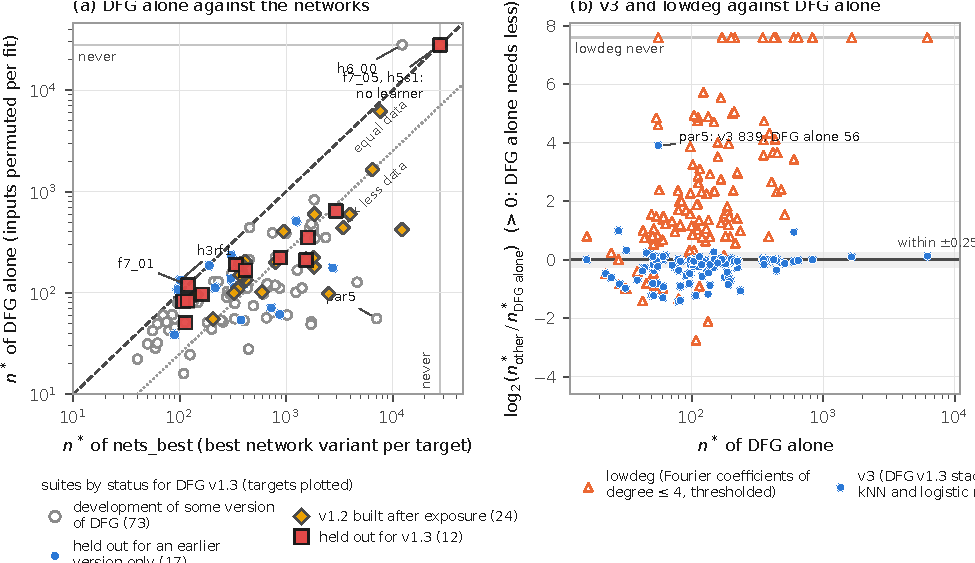
\includegraphics[width=\linewidth]{figures/fig_nstar.pdf}
\caption{(a) $\nstar$ of DFG alone against \code{nets_best} for the 126 targets of the 10 toy suites with network runs \status{Numerical}; colour and marker give the suite's status for DFG v1.3, with \code{dlheld7} as large outlined squares, and ``never'' is drawn at the edge. Below the dashed line DFG needs less data than the best network variant, below the dotted line at least $4\times$ less. (b) For the 134 targets of all 11 suites that DFG alone learns, the $\log_2$ ratio of v3's and of \code{lowdeg}'s $\nstar$ to DFG alone's, against DFG alone's $\nstar$; above 0 DFG alone needs less data; grey: the tie band $\pm0.25$; \code{lowdeg}'s ``never'' at the top. Source: \repo{study/part11/RESULTS.json} via \repo{paper_dfg/make_figures.py}; the plotted points are in \repo{paper_dfg/figures/fig_nstar.json}.}
\label{fig:nstar}
\end{figure}

\paragraph{Pooled} \status{Numerical}.
\begin{itemize}
\item \emph{Against \code{nets_best}:} on the 126 targets of the 10 suites with network runs, DFG's mean is $-1.87$ over the 123 targets both learn, about $3.7\times$ less data (median $-1.65$). Without the held-out \code{dlheld7}, over the 114 in-sample targets, it is $-1.93$ over the 112 both learn. It is clearly better on 117, clearly worse on 2, and needs at least $4\times$ less data on 47 (\cref{fig:nstar}a).
\item \emph{Against single variants:} $-2.04$ against \code{nets_wd}, the one variant run on every suite with network runs (clearly better on 119 of 126, worse on 1), and $-2.64$ against \code{nets} (square loss; 9 suites, 114 targets).
\item \emph{The seven \code{dlheld} suites that Part 10 pooled} (\code{dlheld}, \code{dlheld2}, \dots, \code{dlheld7}, without \code{dlsymdev} and \code{dlfamdev}; 77 targets; for v1.3 only \code{dlheld7} among them is held out): DFG alone is at $-1.71$ and v3 at $-1.87$ against \code{nets_best} on the same targets.
\end{itemize}

\paragraph{By suite} \status{Numerical}. The suite means against \code{nets_best} range from $-2.49$ (\code{dlheld5}) to $-1.27$ (\code{dlheld6}); \code{dlheld7} is at $-1.29$. They are not comparable across suites, because \code{nets_best} minimizes over 2 to 5 variants depending on the suite. Against \code{nets_wd} alone, the three smallest margins are those of the held-out suite and of the two suites held out for v1.1: \code{dlheld2} ($-1.59$), \code{dlheld3} ($-1.60$) and \code{dlheld7} ($-1.62$); the five development suites with network runs give $-1.71$ (\code{dlheld6}) to $-2.45$ (\code{dlsymdev}), and the two exposed suites $-2.05$ and $-2.72$.

\emph{Reading} \status{Heuristic}. Some selection in DFG's favour on the suites it was developed on or exposed to is therefore likely. The suites also differ in kind, though. \code{designed} and \code{random} are small juntas and formulas, \code{dlsymdev} is symmetric, and \code{dlheld2}, \code{dlheld3} and the blind family mix sums, formulas and halfspaces. With 7 to 12 targets per suite, the data do not separate the two explanations. On the held-out suite the margin is about $3\times$ (against \code{nets_wd}), not the $4\times$ of the pooled numbers.

\paragraph{Where DFG is not better} \status{Numerical}. On 9 of the 126 targets with network runs DFG is not clearly better than \code{nets_best}: it is clearly worse on the random formula h3rf1 and on the residue class h6\_00, ties on five (three threshold-like targets, a formula and and3), and no learner learns f7\_05 or h5s1. DFG never learns 4 of the 138 targets (three residue classes mod 3, and h5s1), and neither do v3 and \code{lowdeg} (\cref{app:notwins}). \emph{Reading} \status{Heuristic}: on the small formulas, which v3 and \code{hgb} learn faster, DFG's lack of a clear margin reflects its slowness at small $n$ more than a strength of the networks.

% ------------------------------------------------------------------------------------------------------------------
\subsection{What the portfolio added}\label{sec:res-v3}

On the same training sets and column orders (\cref{sec:refs}; tables in \cref{app:v3}) \status{Numerical}: over the 138 targets, DFG alone's $\nstar$ is lower than v3's on 32 and higher on 101; it equals v3's on 1 (par2), and neither learns 4. Beyond $\pm0.25$ it is lower on 6 and higher on 42. The mean ratio is $+0.19$, so DFG alone needs $1.14\times$ v3's data, and the median is $+0.07$; a two-sided sign test over the 133 targets with unequal $\nstar$ gives $p=1.6\times10^{-9}$. The gap is at small $n$: on the 45 targets that v3 learns by $n=64$, DFG alone's mean is $+0.39$, and v3's test error is lower by more than 0.02 on 63, 64 and 67 of the 138 targets at $n=16$, 32 and 64, on 38 at $n=128$, 17 at 256 and 5 at 512, and on none at $n\ge1024$.
\emph{Reading} \status{Numerical, then Heuristic}. At small $n$ the portfolio's other members carry v3: in Part 10's seed-0 refits the stacker gave the DFG members no weight in 52, 47 and 30 fits at $n=16$, 32 and 64, and on formulas and small thresholds trees, nearest neighbours and logistic regression reach low error with fewer points than DFG needs before its tests admit features. From $n=256$ on, v3 is never worse than its DFG member by more than 0.02, and the DFG members take most of the weight. The reverse, on 3 of the 6 targets where DFG alone needs clearly less data (par3, rf11, par5), is structure that only a fit on all $n$ rows finds: DFG's degree-3 and higher searches need a minimum number of rows and a share of the budget that v3's out-of-fold DFG fits do not have (\cref{app:v3}).

% ------------------------------------------------------------------------------------------------------------------
\subsection{The low-degree algorithm: DFG's characters and test, nothing else}\label{sec:res-lowdeg}

\code{lowdeg} has DFG's global characters up to degree 4 and the same form of union-bound test, applied to the labels, and none of the rest of DFG (\cref{sec:refs}; table in \cref{app:lowdeg}); \cref{fig:nstar}b shows it target by target.

\paragraph{Results} \status{Numerical}.
\begin{itemize}
\item \emph{Against DFG:} pooled over the 138 targets, \code{lowdeg} needs more data. Its mean ratio is $+1.64$ over the 122 targets both learn, about $3.1\times$ more data (median $+1.35$). It is clearly worse on 112 targets and clearly better on 16.
\item \emph{Against the networks} \code{lowdeg} is about even: $-0.16$ against \code{nets_best} over the 112 of 126 targets both learn, clearly better on 53 and clearly worse on 62.
\item \emph{Never learned.} \code{lowdeg} never learns 16 targets: the four that DFG misses and 12 that DFG learns. Of those 12, par5 has degree 5 and is outside \code{lowdeg}'s dictionary; the other 11 are functions of a signed sum, mostly with arbitrary accept sets.
\item \emph{Where \code{lowdeg} is faster.} All 16 such targets are learned at small $n$: DFG needs 22--133 points, \code{lowdeg} 16--61, as on the formulas h3rf0 and h3rf1 and on par4 (28 against 52).
\end{itemize}

\emph{Reading} \status{Heuristic}. DFG's margin over the networks is not explained by its characters and test alone: with them but none of the rest, \code{lowdeg} is at par with the networks. The margin needs what \code{lowdeg} lacks, and the sum blocks are one part of it. They make the signed-sum targets much cheaper to learn, and a few learnable at all within the grid: \code{lowdeg} still learns 39 of the 54 sum-structured targets, more slowly, while DFG without its sum blocks (\code{nosums}, \cref{sec:abl-single}) needs $+0.91$ more in mean $\log_2\nstar$ on the ablation suites and no longer learns band11, h6\_01 and f7\_08. A function of a $k$-input signed sum spreads its Fourier weight over many characters of several degrees, each too weak to pass its own test, while DFG tests the whole block with one $\chi^2$ statistic; the residual rounds let weaker features pass once the stronger ones are fit. On small formulas the comparison runs the other way: at $n\le128$, \code{lowdeg}'s slightly more lenient test, applied to every degree at once on the labels, admits characters at sizes where DFG still keeps few or none.

% ------------------------------------------------------------------------------------------------------------------
\subsection{Input dimension}\label{sec:res-dscale}

DFG and the networks \code{nets} (square loss, the only variant run at every $d$) were run on 7 \code{designed} targets at $d=15$ and 60 and on 4 of them at $d=120$, with seeds 0 and 1, and at $d=30$ with seeds 0, 1 and 2 (\cref{sec:tasks,sec:metrics}). The networks were trained for 20000 steps, 40000 at $d=120$, so one network run, and with it DFG's budget, is twice as large there. \Cref{fig:dscale} plots $\nstar$ with the fitted exponents, and \cref{app:dscale} tabulates them.

\begin{figure}[t]
\centering
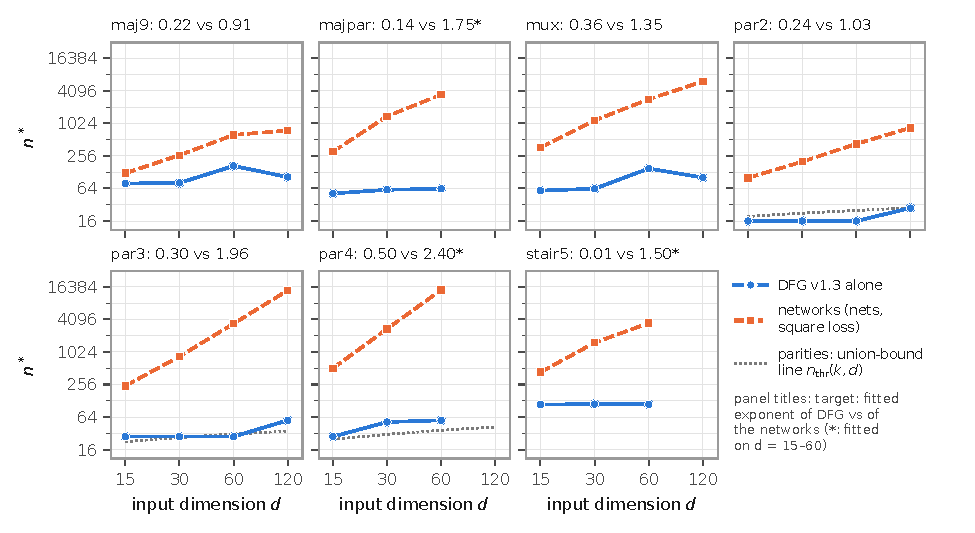
\includegraphics[width=\linewidth]{figures/fig_dscale.pdf}
\caption{$\nstar$ against $d$ (log--log) on the \code{designed} targets with network runs at $d=15$, 60 and 120 (\cref{tab:dscale}) \status{Numerical}. Panel titles give the fitted exponent of DFG v1.3 alone and of the networks \code{nets} ($^\ast$: fitted on $d=15$--60). Dotted, for the $k$-parities: the union-bound line $n_{\rm thr}(k,d)=2\ln(4K\binom{d}{k}/\delta)$ with DFG's $K=4$, $\delta=0.1$ and $c=1$; on the $n$-grid DFG's test passes, when $\bar y$ is near 0, at the first grid point above it (\cref{prop:parity}; where this simple rule misses, and why, is in \cref{app:proof-parity}). Seeds: 2 at $d\ne30$, 3 at $d=30$; the $d=120$ networks were trained for 40000 steps. Source: \repo{study/part11/RESULTS.json} (\texttt{q4\_dscale}) via \repo{paper_dfg/make_figures.py}; the plotted values and $n_{\rm thr}$ are in \repo{paper_dfg/figures/fig_dscale.json}.}
\label{fig:dscale}
\end{figure}

\paragraph{Results} \status{Numerical}.
\begin{itemize}
\item \emph{Exponents.} The least-squares slope of $\log\nstar$ on $\log d$ is 0.01 (stair5) to 0.50 (par4) for DFG v1.3 alone, and 0.91 (maj9) to 2.40 (par4) for the networks, fitted per target on the same $d$.
\item \emph{The gap widens with $d$.} The median $\log_2$ ratio of DFG v1.3 to the networks is $-2.64$ at $d=15$ ($6.2\times$ less data), $-4.19$ at $d=30$ ($18.3\times$), $-4.99$ at $d=60$ ($31.7\times$) and $-5.41$ at $d=120$ ($42.5\times$, 4 targets).
\item \emph{Parities.} DFG's $\nstar$ follows the union-bound line (\cref{fig:dscale}). $n_{\rm thr}$ grows from 19.5 to 27.9 for par2 and from 22.4 to 35.2 for par3 between $d=15$ and 120, and from 24.6 to 36.3 for par4 between $d=15$ and 60. On the grid, DFG's $\nstar$ moves by at most one grid step over the range.
\item \emph{Compute.} DFG's largest fit on these targets uses 0.07, 0.15, 0.18 and 0.18 of one network run at $d=15$, 30, 60 and 120.
\item \emph{The price} \status{Proved, by the code; Numerical}. The enumeration is paid for in FLOPs: an exhaustive degree-$k$ search costs of order $n\binom dk$ FLOPs (\cref{prop:compute}). Within DFG's fixed budget, at $n>512$, the global search can therefore pass no degree-4 character from $d=179$ on and no degree-3 character from $d=630$ on (\cref{prop:floor}; \cref{app:proof-parity,sec:disc-why}).
\end{itemize}

\emph{Reading} \status{Heuristic}.
\begin{itemize}
\item \emph{DFG against gradient descent.} DFG's data cost on a $k$-parity is the union bound's, $2\ln(4K\binom{d}{k}/\delta)$, which grows like $2k\ln d$. The networks' exponents grow with the parity's degree, 1.03, 1.96 and 2.40 for $k=2$, 3 and 4 (par4 fitted on $d=15$--60), as analyses of gradient training on sparse parities lead one to expect \cite{barak2022hidden,abbe2023leap}: exhaustive enumeration pays a logarithm of the dictionary's size, gradient descent a power of $d$.
\item \emph{The size of the factors.} The comparison is with \code{nets}, the plain square-loss network and the weakest variant at $d=30$: on \code{designed}, DFG is at $-2.82$ against \code{nets} and $-2.17$ against \code{nets_wd} (\cref{tab:suites}). The factors are therefore larger than they would be against the best variant. The exponents should be less sensitive to the choice of variant than the factors, but only \code{nets} was run at $d\ne30$.
\end{itemize}

% ------------------------------------------------------------------------------------------------------------------
\subsection{Tabular data and compute}\label{sec:res-tabular}\label{sec:res-compute}

\paragraph{Tabular data} \status{Numerical}. On kr\_vs\_kp and mushroom, the two tabular datasets it can run on (9 cells), DFG is level with gradient boosting in all 9 cells, and with the regularized MLPs and v3 except at the smallest $n$ of kr\_vs\_kp (14.06\% test error against 7.80\% for \code{mlp_reg} and 6.88\% for v3), where they are clearly better; it is nowhere clearly better than the best MLP. Nine cells, with errors near 0 from $n=1000$ on, resolve little. No fit uses more than 0.144 of the standard-task budget. Real-valued data, where Part 7's adaptations of DFG v1.1 were behind a regularized MLP, are not covered (\cref{app:tabular}; \cref{sec:disc-fail}).

\paragraph{Compute} \status{Numerical}. Over all 4730 fits (4334 at $d=30$, 396 at $d\ne30$), the largest uses 0.519 of one network run (h5s5 on \code{dlheld5} at $n=16384$), and none exceeds 0.75. The median fit uses less than 0.001 of a run at $n\le32$, 0.025--0.055 at $n=64$--512 and 0.149 at $n=16384$. CPU time is largest at $n=64$--512 (median 4.2--7.3 seconds per fit), where the cross-validation fits $2F$ small models, each with its own block search. On rough measurements of the same fits DFG alone is faster than v3 (median per-fit CPU ratio 0.06--0.92 at every $n$). Each network fit spends one run by definition, and \code{nets_best} is a hindsight choice among 2 to 5 such runs per target, so ``no more FLOPs'' holds with a wide margin (\cref{app:compute}).
